\documentclass[pdftex,12pt,a4paper]{article}

\usepackage{amsmath}
\usepackage{graphicx}
\usepackage{tikz}
\usepackage[utf8]{inputenc}
\usetikzlibrary{calc}
\usetikzlibrary{decorations.pathmorphing}

\newcommand{\HRule}{\rule{\linewidth}{0.5mm}}
%\renewcommand{\thesection}{\arabic{section}} %Use this when using {report} document class and suffer 0.1 sectioning numbering

\usepackage{listings}
\usepackage{color}

\definecolor{dkgreen}{rgb}{0,0.6,0}
\definecolor{gray}{rgb}{0.5,0.5,0.5}
\definecolor{mauve}{rgb}{0.58,0,0.82}

\lstset{frame=tb,
  language=C,
  aboveskip=3mm,
  belowskip=3mm,
  showstringspaces=false,
  columns=flexible,
  basicstyle={\small\ttfamily},
  numbers=none,
  numberstyle=\tiny\color{gray},
  keywordstyle=\color{blue},
  commentstyle=\color{dkgreen},
  stringstyle=\color{mauve},
  breaklines=true,
  breakatwhitespace=true,
  tabsize=4
}

\pdfinfo {
			   /Title  (Robotic Arm Simulating Pre-Thesis)
               /Creator (Nguyen Vu Hoi)
               /Author (Nguyen Vu Hoi vuhoinguyen@gmail.com)
               /CreationDate (D:20030101000000)  %format D:YYYYMMDDhhmmss
               /ModDate (D:20030815213532)
               /Subject (Writing a Bachelor pre-thesis about simulation and controlling robotic arm)
               /Keywords (Bachelor, Thesis, Pre-thesis, Robotic, Arm, Gazebo, ROS, Robotics Operating System, Linux, Ubuntu, Vu Hoi Nguyen, VGU, Vietnamese-German University)}
                  
\begin{document}
  \begin{titlepage}
\begin{center}

% Upper part of the page. The '~' is needed because \\
% only works if a paragraph has started.

\includegraphics[width=0.3\textwidth]{./image/vgu_logo}~\\[1cm]
\textsc{\LARGE vietnamese-german university}~\\[0.2cm]
Electrical Engineering and Information Technology Department ~\\[3cm]
\textsc{\Large pre-thesis project}\\[0.5cm]

% Title
\HRule \\[0.4cm]
{ \huge \bfseries Robotic Arm:\\ Simulation on Linux \\ Using Gazebo and ROS \\[0.5cm] }

\HRule \\[3cm]

% Author and supervisor
\noindent
\begin{minipage}[t]{0.4\textwidth}
\begin{flushleft} \large
\emph{Author:}\\
Vu Hoi \textsc{NGUYEN}
\end{flushleft}
\end{minipage}%
\begin{minipage}[t]{0.4\textwidth}
\begin{flushright} \large
\emph{Supervisor:} \\
Prof. ~Peter \textsc{NAUTH} \\
Lab.Eng. Dinh Than \textsc{LE}
\end{flushright}
\end{minipage}
\vfill

% Bottom of the page
~\\[1cm]
{\large \today}

\end{center}

\begin{tikzpicture}[overlay,remember picture]

    \draw [line width=1mm,decorate,decoration={
        }]
        ($ (current page.north west) + (1cm,-1cm) $)
        rectangle
        ($ (current page.south east) + (-1cm,1cm) $);
        
\end{tikzpicture}

\end{titlepage}

  
  \pagenumbering{gobble}
  
  \newpage
  \tableofcontents
  \listoffigures
  
  \newpage
  \pagenumbering{arabic}
  \section*{Abstract}
  This document is written as a requirement of the course "Elective project" for senior year in Vietnamese-German University. It reports the content of the project, my working process, the result and discuss the problems which are frequently occurs in the process.\\
  My project studies the controlling methods providing by Robotics Operating System (ROS) and simulation sequence using Gazebo on Linux (specifically distribution Ubuntu). \\
  The goal of the project is to successfully create a humanoid arm inside Gazebo and control its virtual joints using ROS.\\
  To do this, a virtual-physical model need to be coded using a marking language (xml). A robot is divided in to single "links" (ex. upper arm, forearm, hand, ...), connected by "joints" (ex. elbow, wrist, ...). These links are constructed by the simplest 3D shapes like spheres or boxes for faster and easier simulating. This model also holds the physical properties of the links such as dimensions of the parts, their mass, initials; type of the links (revolve, linear, ...) and relationship between the links and the joints. Gazebo then takes care of the relationships and simulate the behavior of the robot in the virtual environment.\\
  Furthermore, this model must have an appearance which is friendly to users (actual look of the robot, not just basic shapes). This "real" appearance is designed in another software, then exported (and imported into Gazebo) in form of a .stl file. Gazebo, again, take care of this change and display the new appearance of the robot into its 3D environment. \\
  As the last part, "virtual" motors are attached to the joints of the model and controlled by ROS. Although these joints can be controlled directly inside Gazebo, using ROS have a critical importance, as standardized ROS controlling methods can as well be used in other environments (including real life). That way, ROS will significantly reduce the future work if one attends to apply this simulation to a real robot, which is obviously the purpose in doing simulations and will be surely done.\\
  
  \newpage
  \section{Introduction}
  \subsection{Humanoid robotics history}
  Surprisingly, the idea about a humanoid robot is not a modern concept, but has been discussed thousands of years ago. According to the ancient Lie Zi text, Yan Shi made a moving mechanical device resembling a human being in 10th century BC. Year 322 BC, famous philosopher Aristotle talked about a future of human equality, made true using some kind of devices with artificial intelligence:
  
  "There is only one condition in which we can imagine managers not needing subordinates, and masters not needing slaves. This condition would be that each instrument could do its own work, at the word of command or by intelligent anticipation, like the statues of Daedalus or the tripods made by Hephaestus, of which Homer relates that "Of their own motion they entered the conclave of Gods on Olympus", as if a shuttle should weave of itself, and a plectrum should do its own harp playing."\\
  Later on, in first century AD, Hero of Alexandria created many automatons, including ones that could speak. Then in 1495, Leonardo Da Vinci created Leonardo's robot, which could be referred as the first real humanoid robot. It is a mechanical knight, clad in medieval armor. Its joints are designed so that it can sit up, wave arms, move its head and open or close its jaw.
  \begin{figure}[h]
      \centering
      %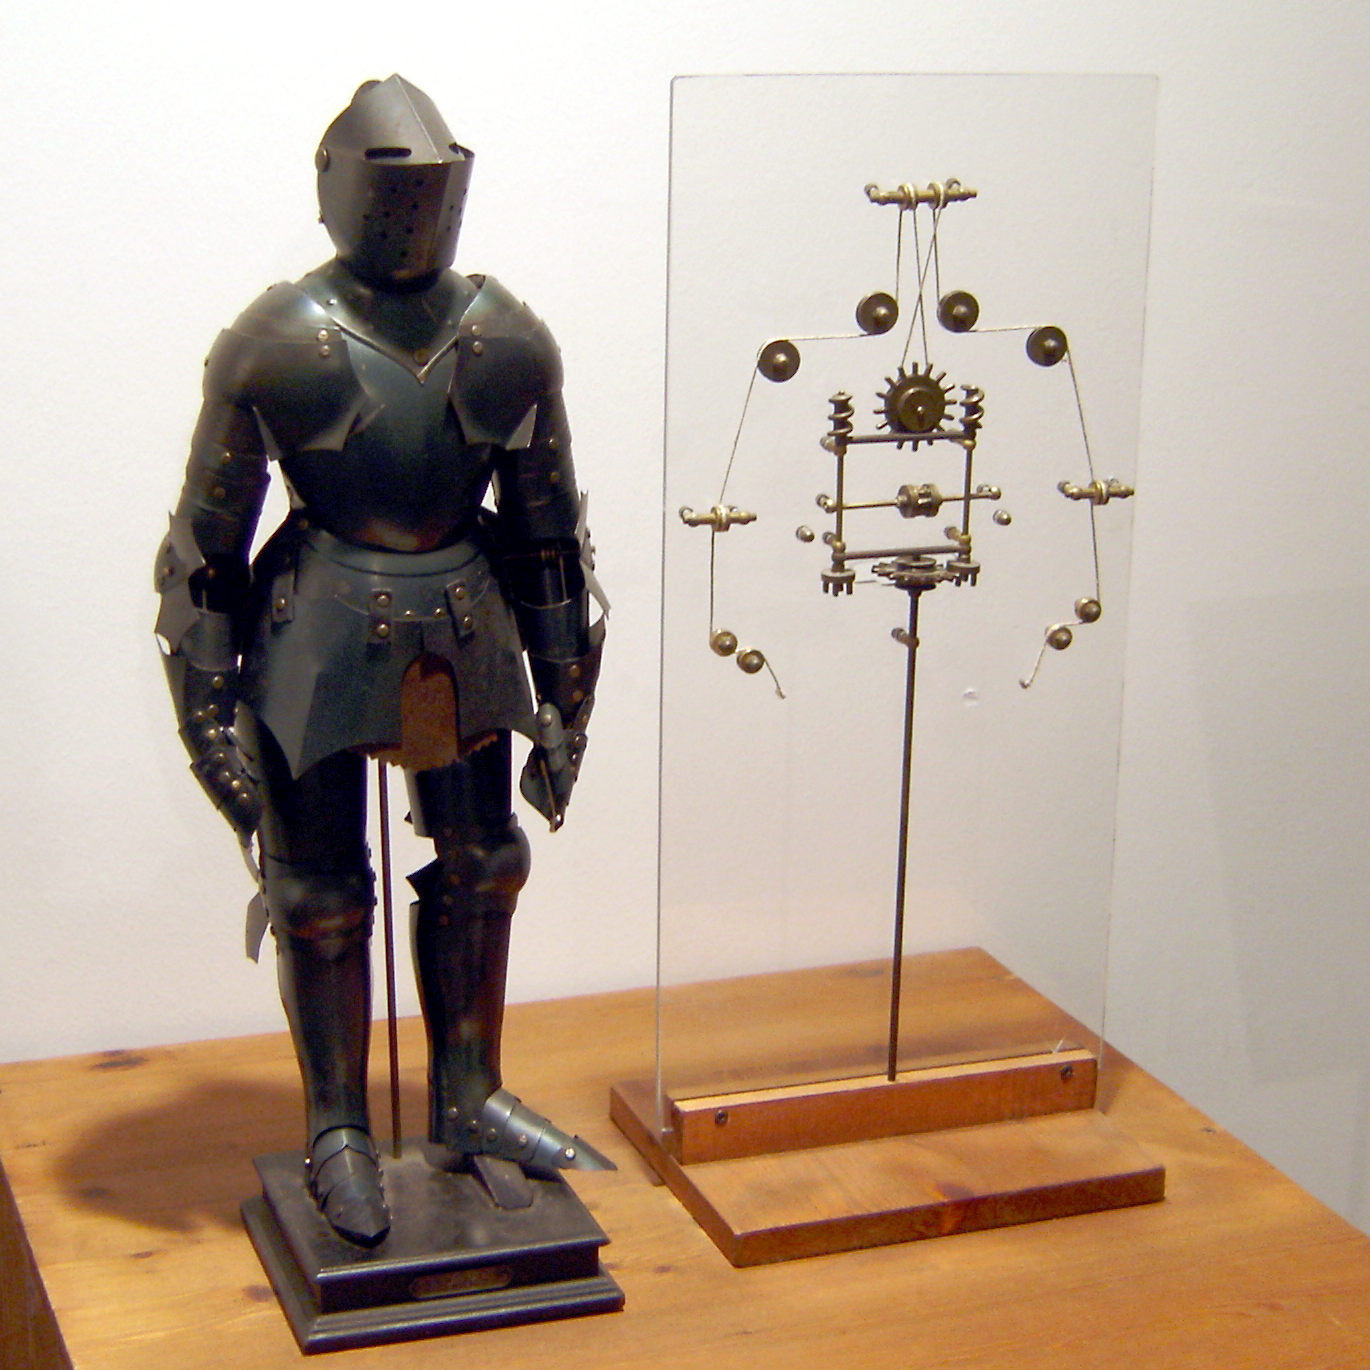
\includegraphics[width=0.55\linewidth]{image/Leonardo-Robot3}
      \caption{Model of Leonardo's robot with inner workings, displayed in Berlin}
      \label{fig:leonardo_robot}
  \end{figure}
  
  \newpage
  With its potential, humanoid robotics develops faster and faster, more and more designs and definitions are published. In 1921, the term "robot" was initially used in the play "Rossum's Universal Robots". In 1941, a scientist and a science fiction writer, Isaac Asimov, first used the word "robotics" as the description of the study and use of robots, foreseeing the development of robot industry. 
  In 1928, engineer W. H. Richards created Eric robot, which exhibited in London its basic functions like moving its hands and head, controlled by remote control or by voice.
  \begin{figure}[h]
        \centering
        %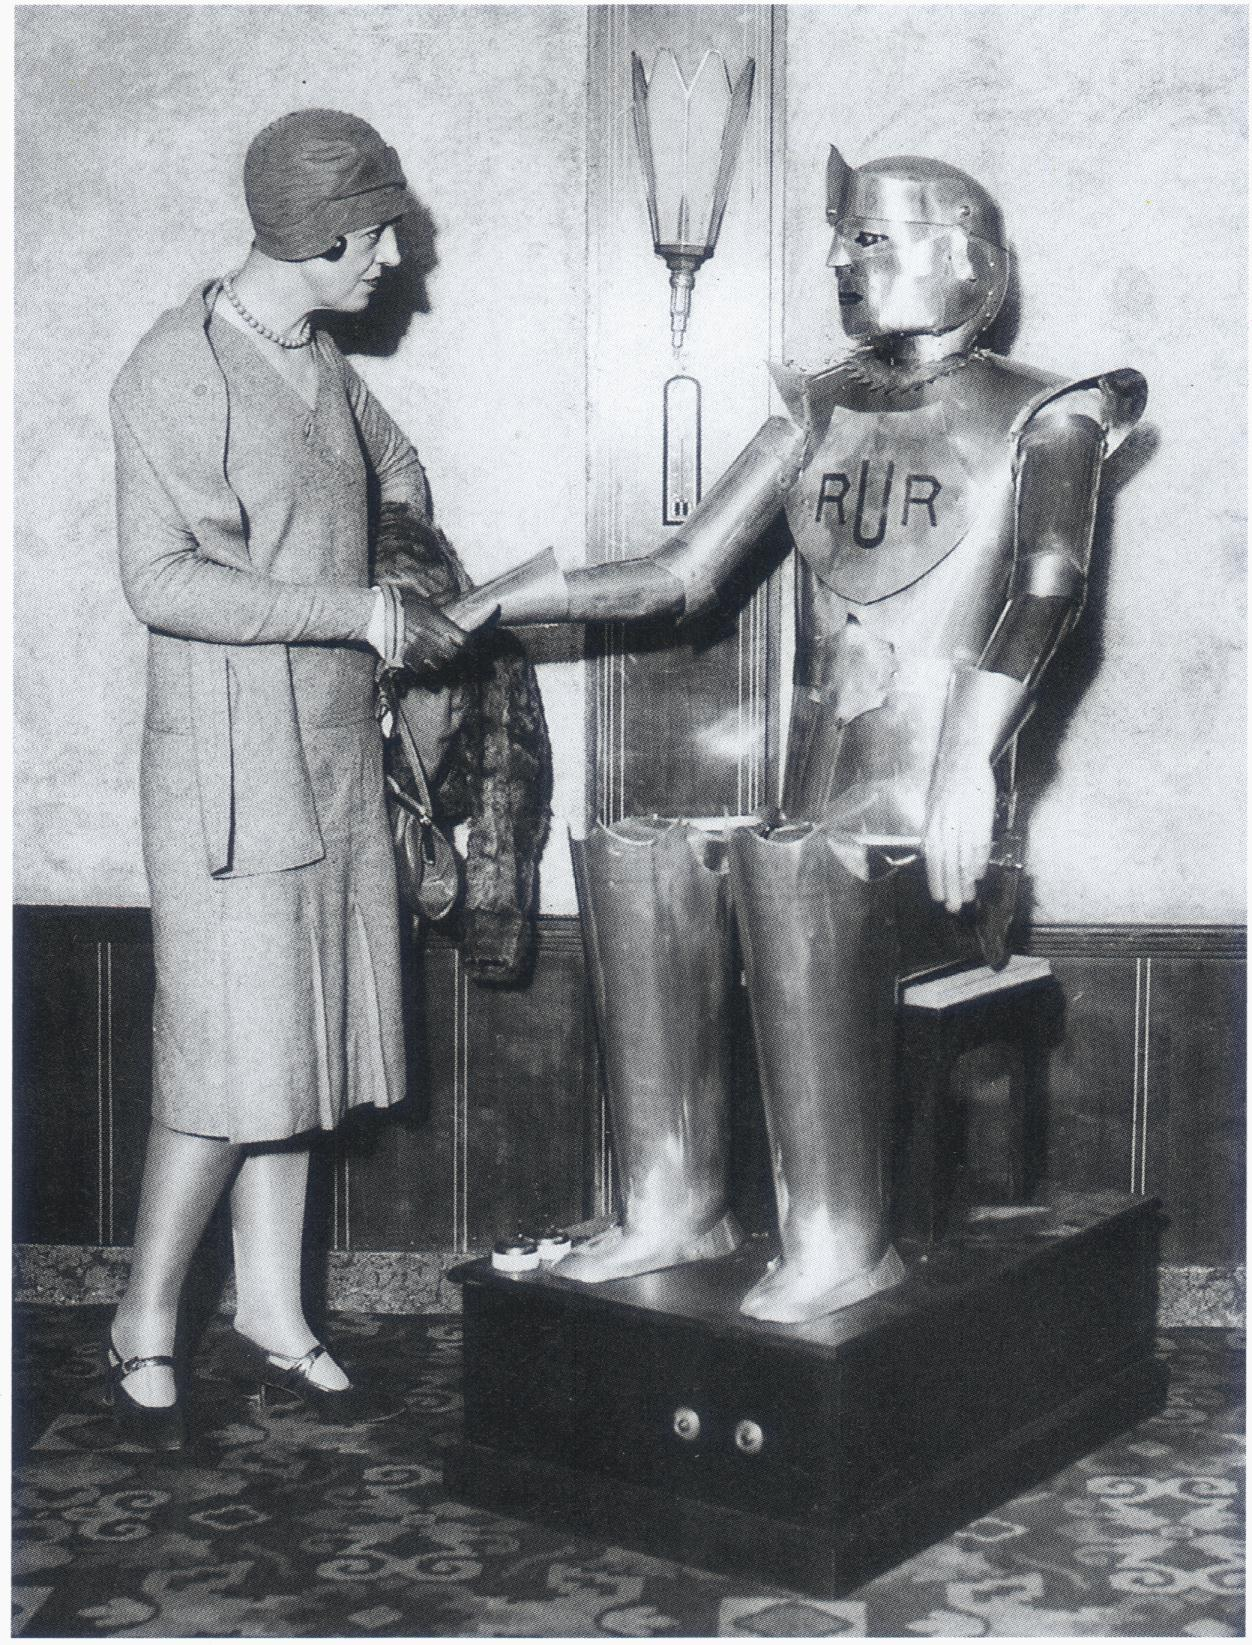
\includegraphics[width=0.55\linewidth]{image/Eric_DRKp2.jpg}
        \caption{ERIC robot, showed in 1928}
        \label{fig:eric_robot}
  \end{figure} \\
  1948, W. Grey Walter created turtles robots called Elmer and Elsie, which are capable of finding their charging station when they are out of power. \\
  1956, George Devol and Joseph Engelberger together founded 'Unimation', the very first robot company. Engelberger, who is also widely known as 'father of robotics’, made a significant turn in robot history and promoted the rise of programmable robots all over the world. \\
  1964, AI research labs were opened at MIT, Stanford University and the University of Edinburgh. \\
  1969, Stanford Arm, first successful electrically-powered, computer-controlled robot arm was built by Victor Scheinman. \\
  1973, WABOT I, the first human-scale anthropomorphic robot, was completed. Its system can control its limbs, vision and have simple Japanese conversations. Its "mental ability" is supposed to be similar to a 18 month old child.\\
  1980, WL-9DR robot of Waseda University, Tokyo made its first Quasi-dynamic walking step of the world.\\
  1989, WL12RIII, a product of Kato Corporation, could walk up and down stairs and take a single step every 0.64 seconds.
  \begin{figure}[h]
          \centering
          %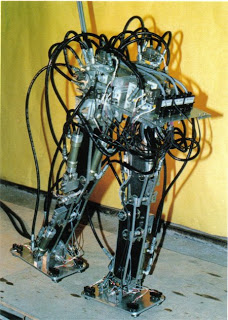
\includegraphics[width=0.55\linewidth]{image/WL-9DR-1980.jpg}
          \caption{WL12RIII biped robot in 1989}
          \label{fig:WL12RIII_robot}
  \end{figure}\\
  2002, Honda created the infamous ASIMO. It is supposed to be an AI assistant. ASIMO is capable of doing complex tasks like recognize its owner, connect with a computer, read email or stream video with its camera. \\
  
  Why we need humanoid robots? \\
  The change in number of humanoid robots. \\
  HR in Vietnam. \\
  \subsection{Why Linux, Gazebo, ROS?}
  
  \newpage
  \section{Working with ROS}
  \subsection{Basic parts of ROS}
  
  \newpage
  \subsection{Publishers and Subscribers}
  
  \newpage
  \section{Gazebo Simulation}
  Abstract
  
  \newpage
  \section{Control Gazebo by ROS}
  Abstract

  \newpage
  \section{Project operating timeline}
  Abstract
  
  \newpage
  \section{Conclusion}
  Abstract
  
  \newpage
  \section{Reference}
  Robot analysis and control Haruhiko Asada, Jean-Jacques E.Slotine
  Introduction to Robotics: Mechanics and Control, John J. Craig, third edition
  http://www.generationrobots.com/en/content/75-gazebo-and-ros
  http://robotica.unileon.es/mediawiki/index.php/MYRAbot%27s_arm_model_for_simulation_%28urdf%2Bgazebo%29
  http://www.robotshop.com/media/files/PDF/timeline.pdf
  http://robotica.unileon.es/mediawiki/index.php/MYRAbot%27s_arm_control_%28bioloid%2Barduino%29
  http://wiki.ros.org/rosserial_arduino/Tutorials/Arduino%20IDE%20Setup
  http://www.cse.sc.edu/~jokane/agitr/agitr-letter-pubsub.pdf
  http://docs.ros.org/indigo/api/roscpp/html/classros_1_1NodeHandle.html#a6b655c04f32c4c967d49799ff9312ac6
  http://www.allonrobots.com/leonardo-da-vinci.html
  https://www.sharelatex.com/learn/
  http://cyberneticzoo.com/robots/1928-eric-robot-capt-richards-english/
  \begin{lstlisting}
  // Hello.cpp
  #include javax.swing.JApplet;
  import java.awt.Graphics;
  
  public class Hello extends JApplet {
	  public void paintComponent(Graphics g) {
          g.drawString("Hello, world!", 65, 95);
      }    
  }
  \end{lstlisting}
  
\end{document}